\documentclass{article}
\usepackage{lmodern}
\usepackage{graphicx}
\usepackage{tikz}
\usepackage{chemfig}
\usetikzlibrary{shapes.geometric, arrows}
\usetikzlibrary{calc}
\tikzstyle{start} = [rectangle, rounded corners, minimum width=2cm, minimum height=1cm,text centered, text width=2cm, draw=black, fill=red!30]
\tikzstyle{io} = [trapezium, trapezium left angle=70, trapezium right angle=110, minimum width=3cm, text centered,text width = 4cm, minimum height=1cm, draw=black, fill=blue!30]
\tikzstyle{process} = [rectangle, minimum width=3cm, minimum height=1cm, text centered, draw=black, fill=orange!30]
\tikzstyle{decision} = [diamond, minimum width=3cm, minimum height=1cm, text centered, draw=black, text width=1.5cm,fill=green!30]
\tikzstyle{position} = [rectangle, minimum width=3cm, minimum height=1cm, text centered, draw=black,fill=blue!20]
\tikzstyle{arrow} = [thick,->,>=stealth]
\begin{document}
\pagenumbering{gobble}
\begin{center}
\scalebox{0.8}{
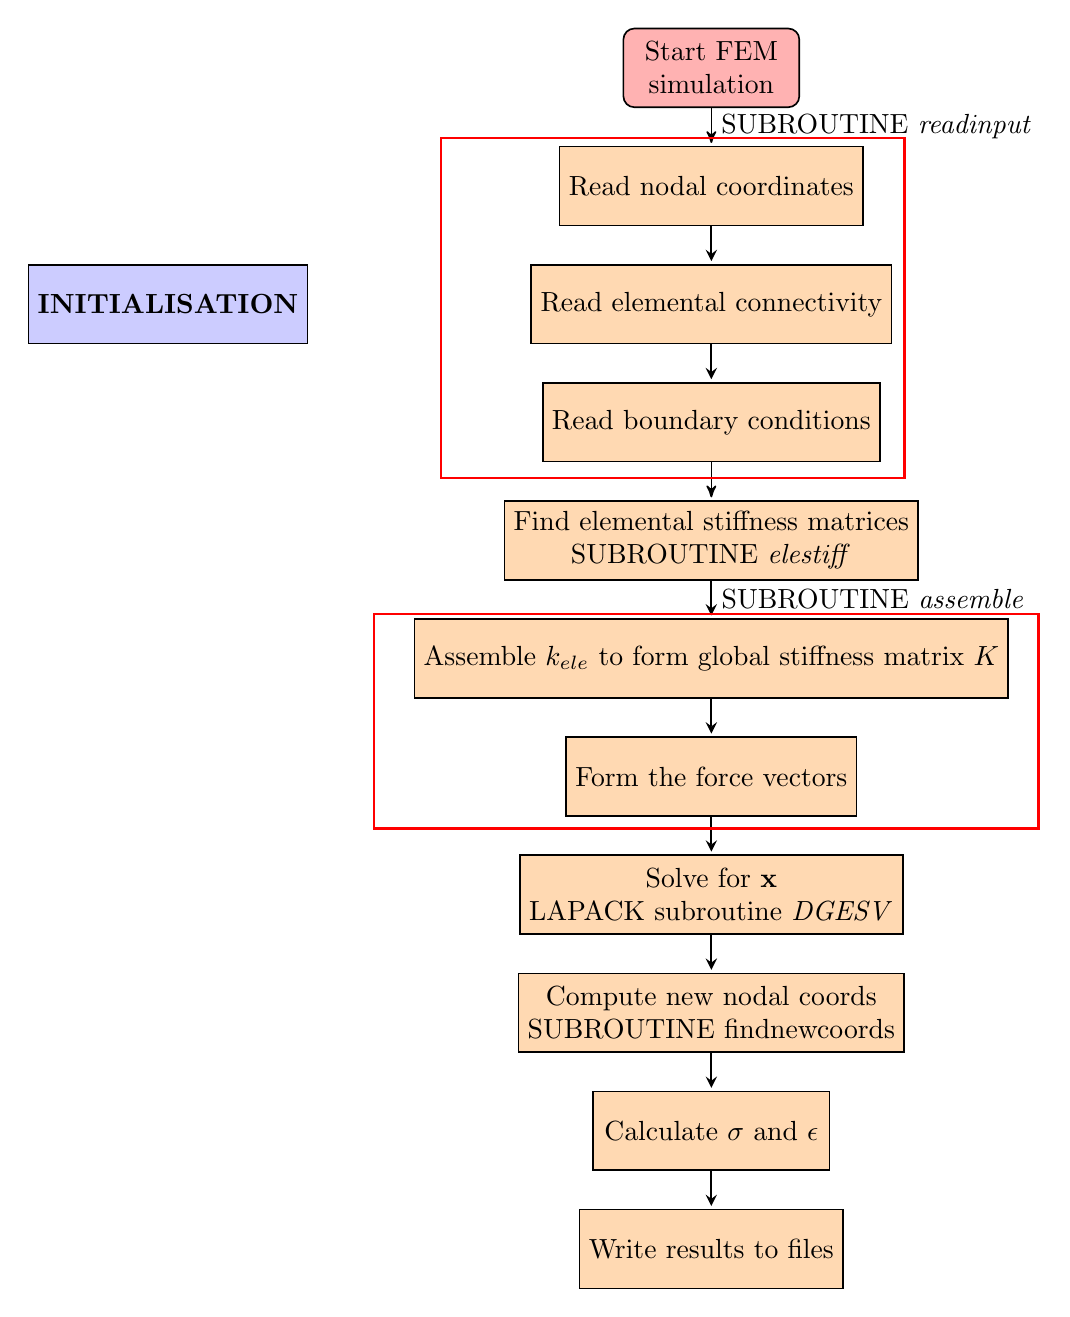
\begin{tikzpicture}[->,>=stealth',shorten >=1pt,auto,node distance=1.5cm,semithick]

\node (start) [start] {Start FEM simulation};
\node (readnode) [process,below of=start] {Read nodal coordinates};
\node (readele) [process,below of=readnode] {Read elemental connectivity};
\node (readbcs) [process,below of=readele] {Read boundary conditions};
\node (elestiff) [process,below of=readbcs,align=center] {Find elemental stiffness matrices \\ SUBROUTINE \emph{elestiff}};
\node (globalstiff) [process,below of=elestiff] {Assemble $k_{ele}$ to form global stiffness matrix $K$};
\node (formforce) [process,below of=globalstiff] {Form the force vectors};
\node (solve) [process,below of=formforce,align=center] {Solve for \textbf{x} \\ LAPACK subroutine \emph{DGESV}};
\node (newcoords) [process,below of=solve,align=center] {Compute new nodal coords \\ SUBROUTINE findnewcoords};
\node (strstr) [process,below of=newcoords] {Calculate $\sigma$ and $\epsilon$};
\node (results) [process,below of=strstr] {Write results to files};


\draw [->] (start) -- node{SUBROUTINE \emph{readinput}} (readnode);
\draw [arrow] (readnode) -- (readele);
\draw [arrow] (readele) -- (readbcs);
\draw [->] (readbcs) -- (elestiff);
\draw [arrow] (elestiff) -- node {SUBROUTINE \emph{assemble}} (globalstiff);
\draw [arrow] (globalstiff) -- (formforce);
\draw [arrow] (formforce) -- (solve);
\draw [arrow] (solve) -- (newcoords);
\draw [arrow] (newcoords) -- (strstr);
\draw [arrow] (strstr) -- (results);

\node (initialise) [position, left of=readele, xshift=-5.4cm] {\textbf{INITIALISATION}} ;

\draw[red,thick] ($(readnode.north west)+(-1.5,0.1)$)  rectangle ($(readbcs.south east)+(0.3,-0.2)$);
\draw[red,thick] ($(globalstiff.north west)+(-0.5,0.05)$)  rectangle ($(formforce.south east)+(2.3,-0.15)$);

\end{tikzpicture}
}
\end{center}
\end{document}
